\documentclass{vegaarticle}

\author{}
\title{Forecasting and Analysing the Yield Curve: An Econometric Study}
\date{}

\addbibresource{refs.bib}

\begin{document}
    \maketitle

    \begin{abstract}{}
        This research study employs econometric analysis techniques to investigate the forecasting of the yield curve, analyze impulse response functions (IRFs), and detect structural breaks. Accurate forecasting of the yield curve is crucial for investors, policymakers, and risk managers in making informed decisions. The analysis of IRFs provides insights into the dynamic response of the yield curve to shocks in macroeconomic variables, allowing for a deeper understanding of the transmission mechanisms. Additionally, the study examines structural breaks in the yield curve associated with unpredictable events, providing valuable insights into shifts in market dynamics. By combining these three components, this research contributes to a broader understanding of the yield curve's behavior and its implications for financial markets and economic policies.
    \end{abstract}

    \introduction
        The yield curve, depicting the relationship between time to maturity and yields on zero-coupon bonds, serves as a vital indicator of market expectations, economic conditions, and future monetary policy. Accurate forecasting of the yield curve has tremendous implications for investors, policymakers, and risk managers. Simultaneously, understanding the dynamic response of the yield curve to shocks and structural breaks enables a deeper comprehension of the underlying economic factors and their impact on financial markets.

        This paper aims to contribute to the existing literature by conducting a comprehensive econometric analysis that encompasses yield curve forecasting, impulse response analysis, and the investigation of structural breaks. By incorporating these three key components, this research seeks to shed light on the interplay between economic variables, forecast future yield curve movements, and detect shifts in the yield curve structure associated with unpredictable events.
        
        The first component of this study focuses on yield curve forecasting using econometric techniques, such as Vector Autoregression (VAR) models or Dynamic Nelson-Siegel (DNS) models. By leveraging historical data on zero-coupon yields and potential explanatory variables, the chosen model will provide forecasts for the yield curve over a specified time horizon. The accuracy of these forecasts will be rigorously evaluated using statistical measures such as mean absolute error (MAE) or root mean squared error (RMSE), allowing for an assessment of the model's predictive capabilities.
        
        In addition to forecasting, this research incorporates the analysis of impulse response functions (IRFs). Through estimating the dynamic response of the yield curve to shocks in relevant macroeconomic variables such as GDP growth, inflation, or monetary policy indicators, the IRFs provide insight into the transmission channels and the lagged effects of these shocks on the yield curve. This analysis will enhance our understanding of the interactions between the yield curve and important economic factors, contributing to the wider field of monetary policy and financial markets.
        
        Furthermore, we address the critical aspect of detecting and studying structural breaks in the yield curve. Unforeseen events, whether political, social, or economic in nature, can lead to significant shifts in the yield curve's structure. By employing robust econometric techniques, such as Chow tests, Bai-Perron tests, or Markov-switching models, this study will identify and examine these structural breaks. The timing, magnitude, and nature of the breaks will be analyzed, providing valuable insights into the factors driving the shifts and their implications for market dynamics.
        
        In summary, this research aims to offer a comprehensive analysis of the yield curve, incorporating yield curve forecasting, impulse response analysis, and the study of structural breaks. By combining these three aspects, we provide insights into the future movements of the yield curve, the dynamic response to macroeconomic shocks, and the detection of structural changes associated with unpredictable events. These findings hold significant implications for investors, policymakers, and market participants, ultimately contributing to a deeper understanding of macroeconomic dynamics and aiding in informed decision-making in financial markets.
            
    \section{Understanding the yield curve}
        \section{Understanding the yield curve}

    \section{Literature Review}
        \section{Literature Review}

    \section{Data Collection and Preprocessing}
        \section{Data Collection and Preprocessing}
We use the Russian Government Bond Zero Coupon Yield Curve, provided by the Moscow Exchange (MOEX), for our research. It is calculated from the curve basis, and the detailed methodology for defining the curve can be found in \cite{MOEXGCURVEdocs}. 

For our analysis, we collected the daily yield curve data spanning from February 1, 2008, to January 30, 2014. The train-test split date we applied is November 15, 2012, to ensure accurate modeling and evaluation. Additionally, to examine a more concentrated time frame, we created a smaller dataset containing monthly data from February 1, 2008, to November 1, 2013.

In Figure \ref{fig:ZCYC}, you can observe the typical behavior of yield curves.
\begin{figure}[htbp]
    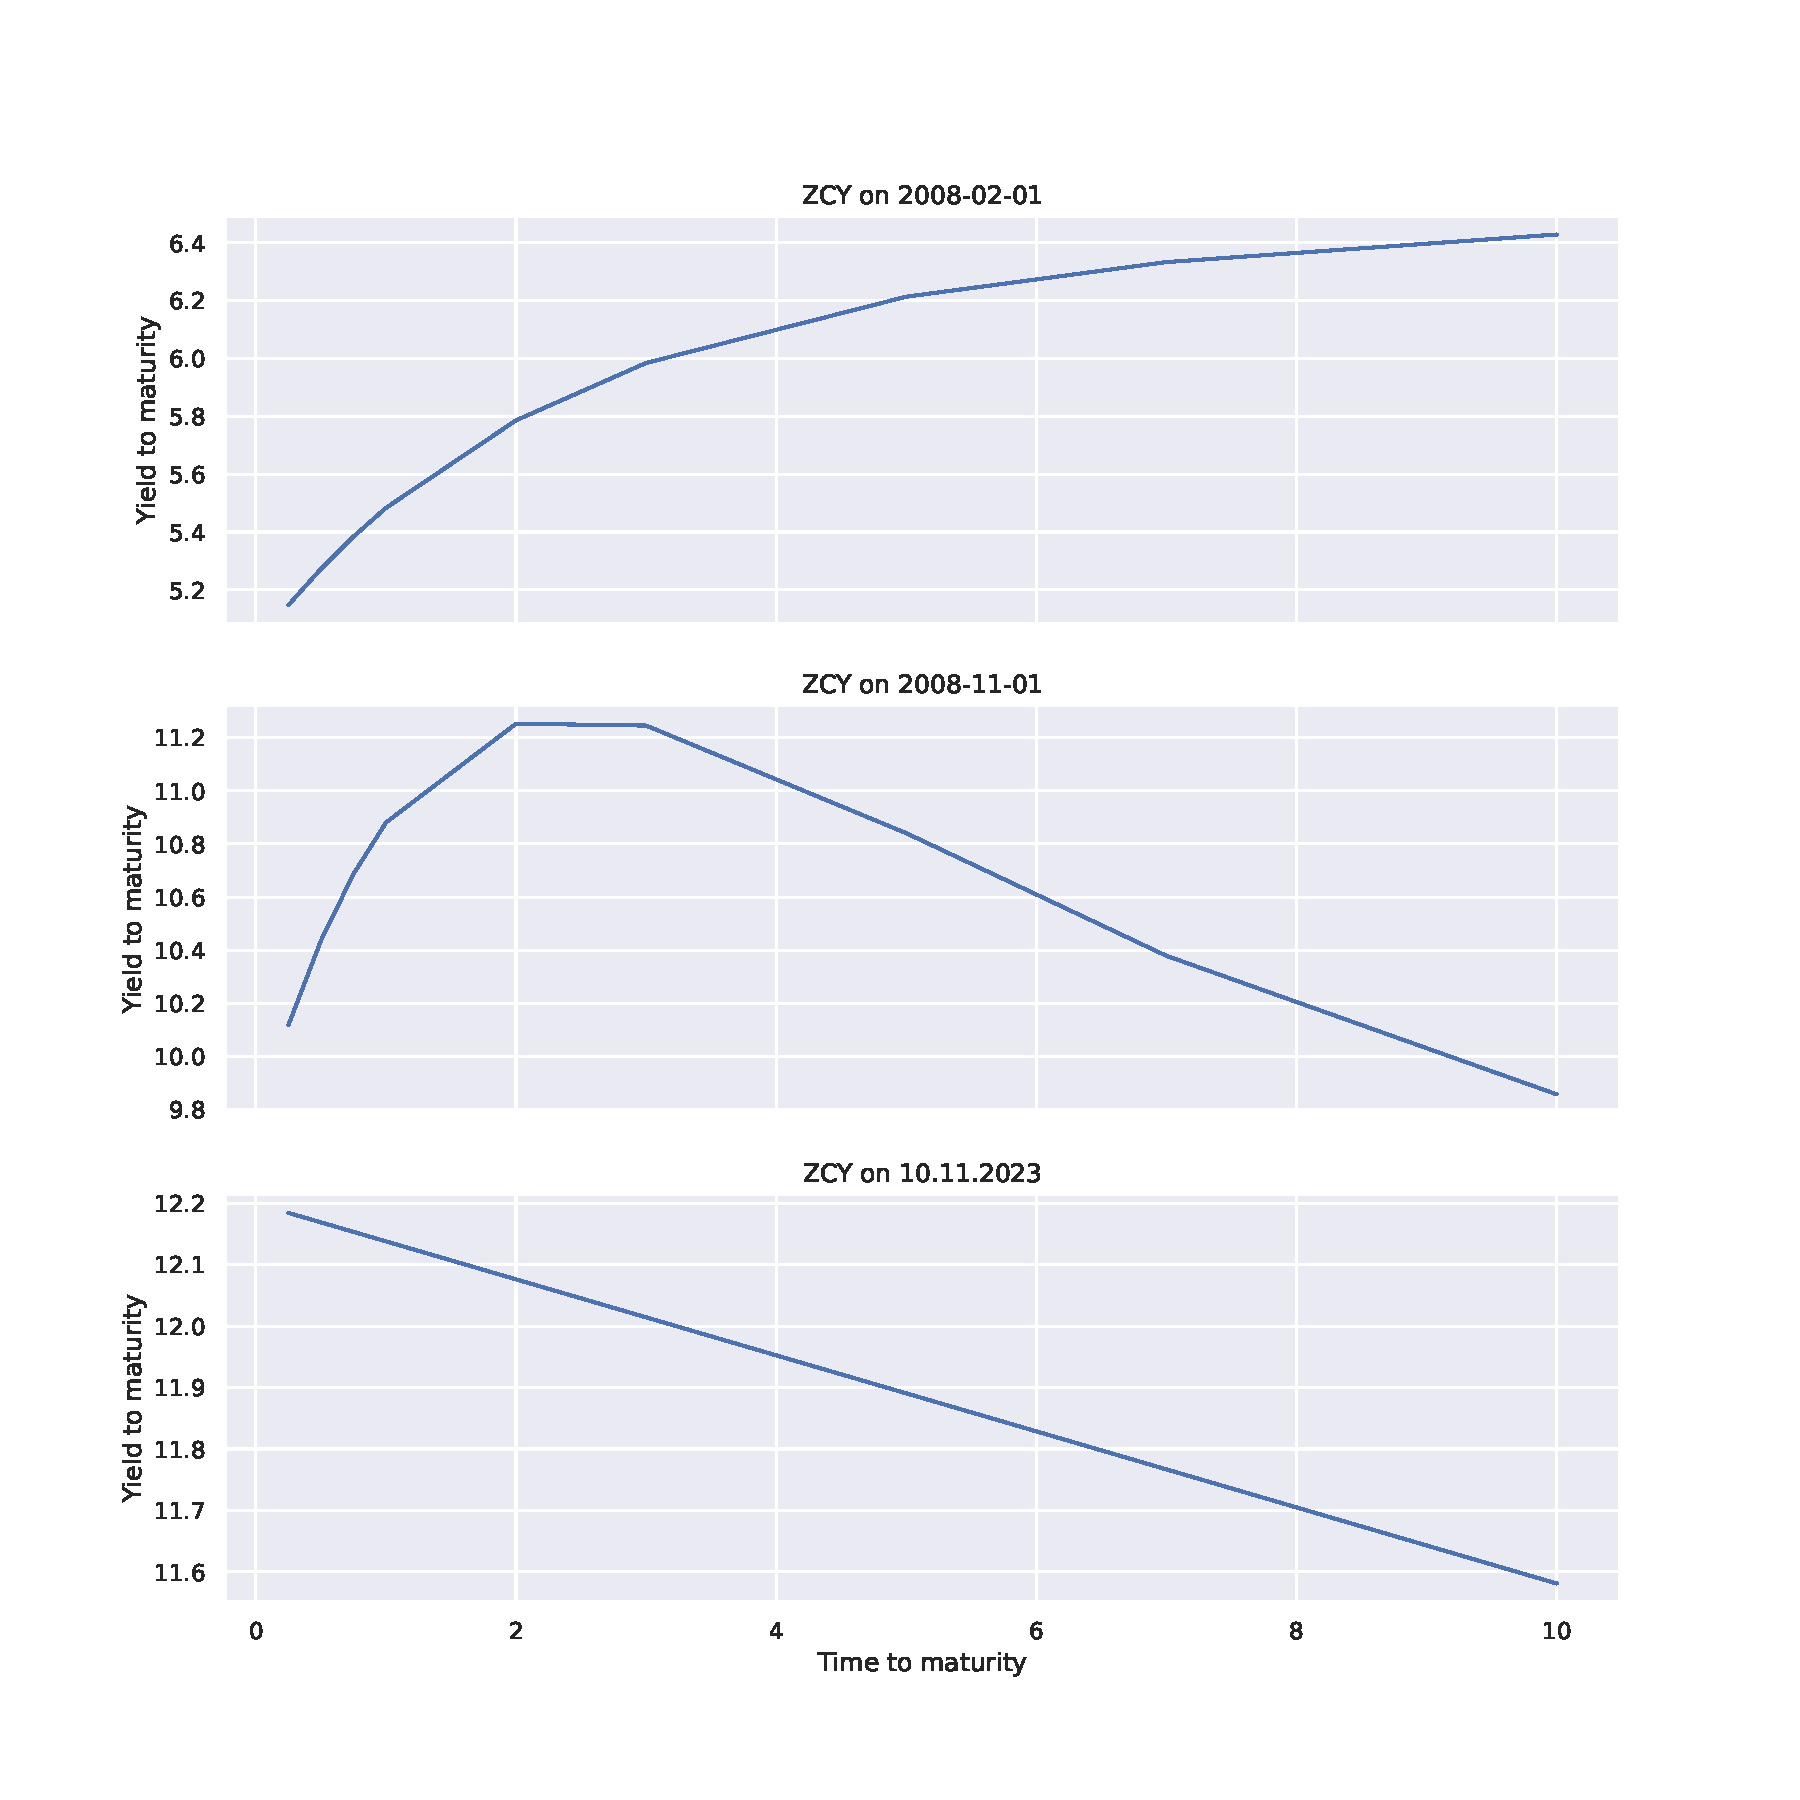
\includegraphics[width=\linewidth]{ZCY.pdf}
    \caption{Russian government bond yield curves}
    \label{fig:ZCYC}
\end{figure}

In Figure \ref{fig:YTMdynamics}, which visualizes the dynamic changes in bond yields, you can observe the typical behavior of short-term, mid-term, and long-term yields based on our analysis.
\begin{figure}[htbp]
    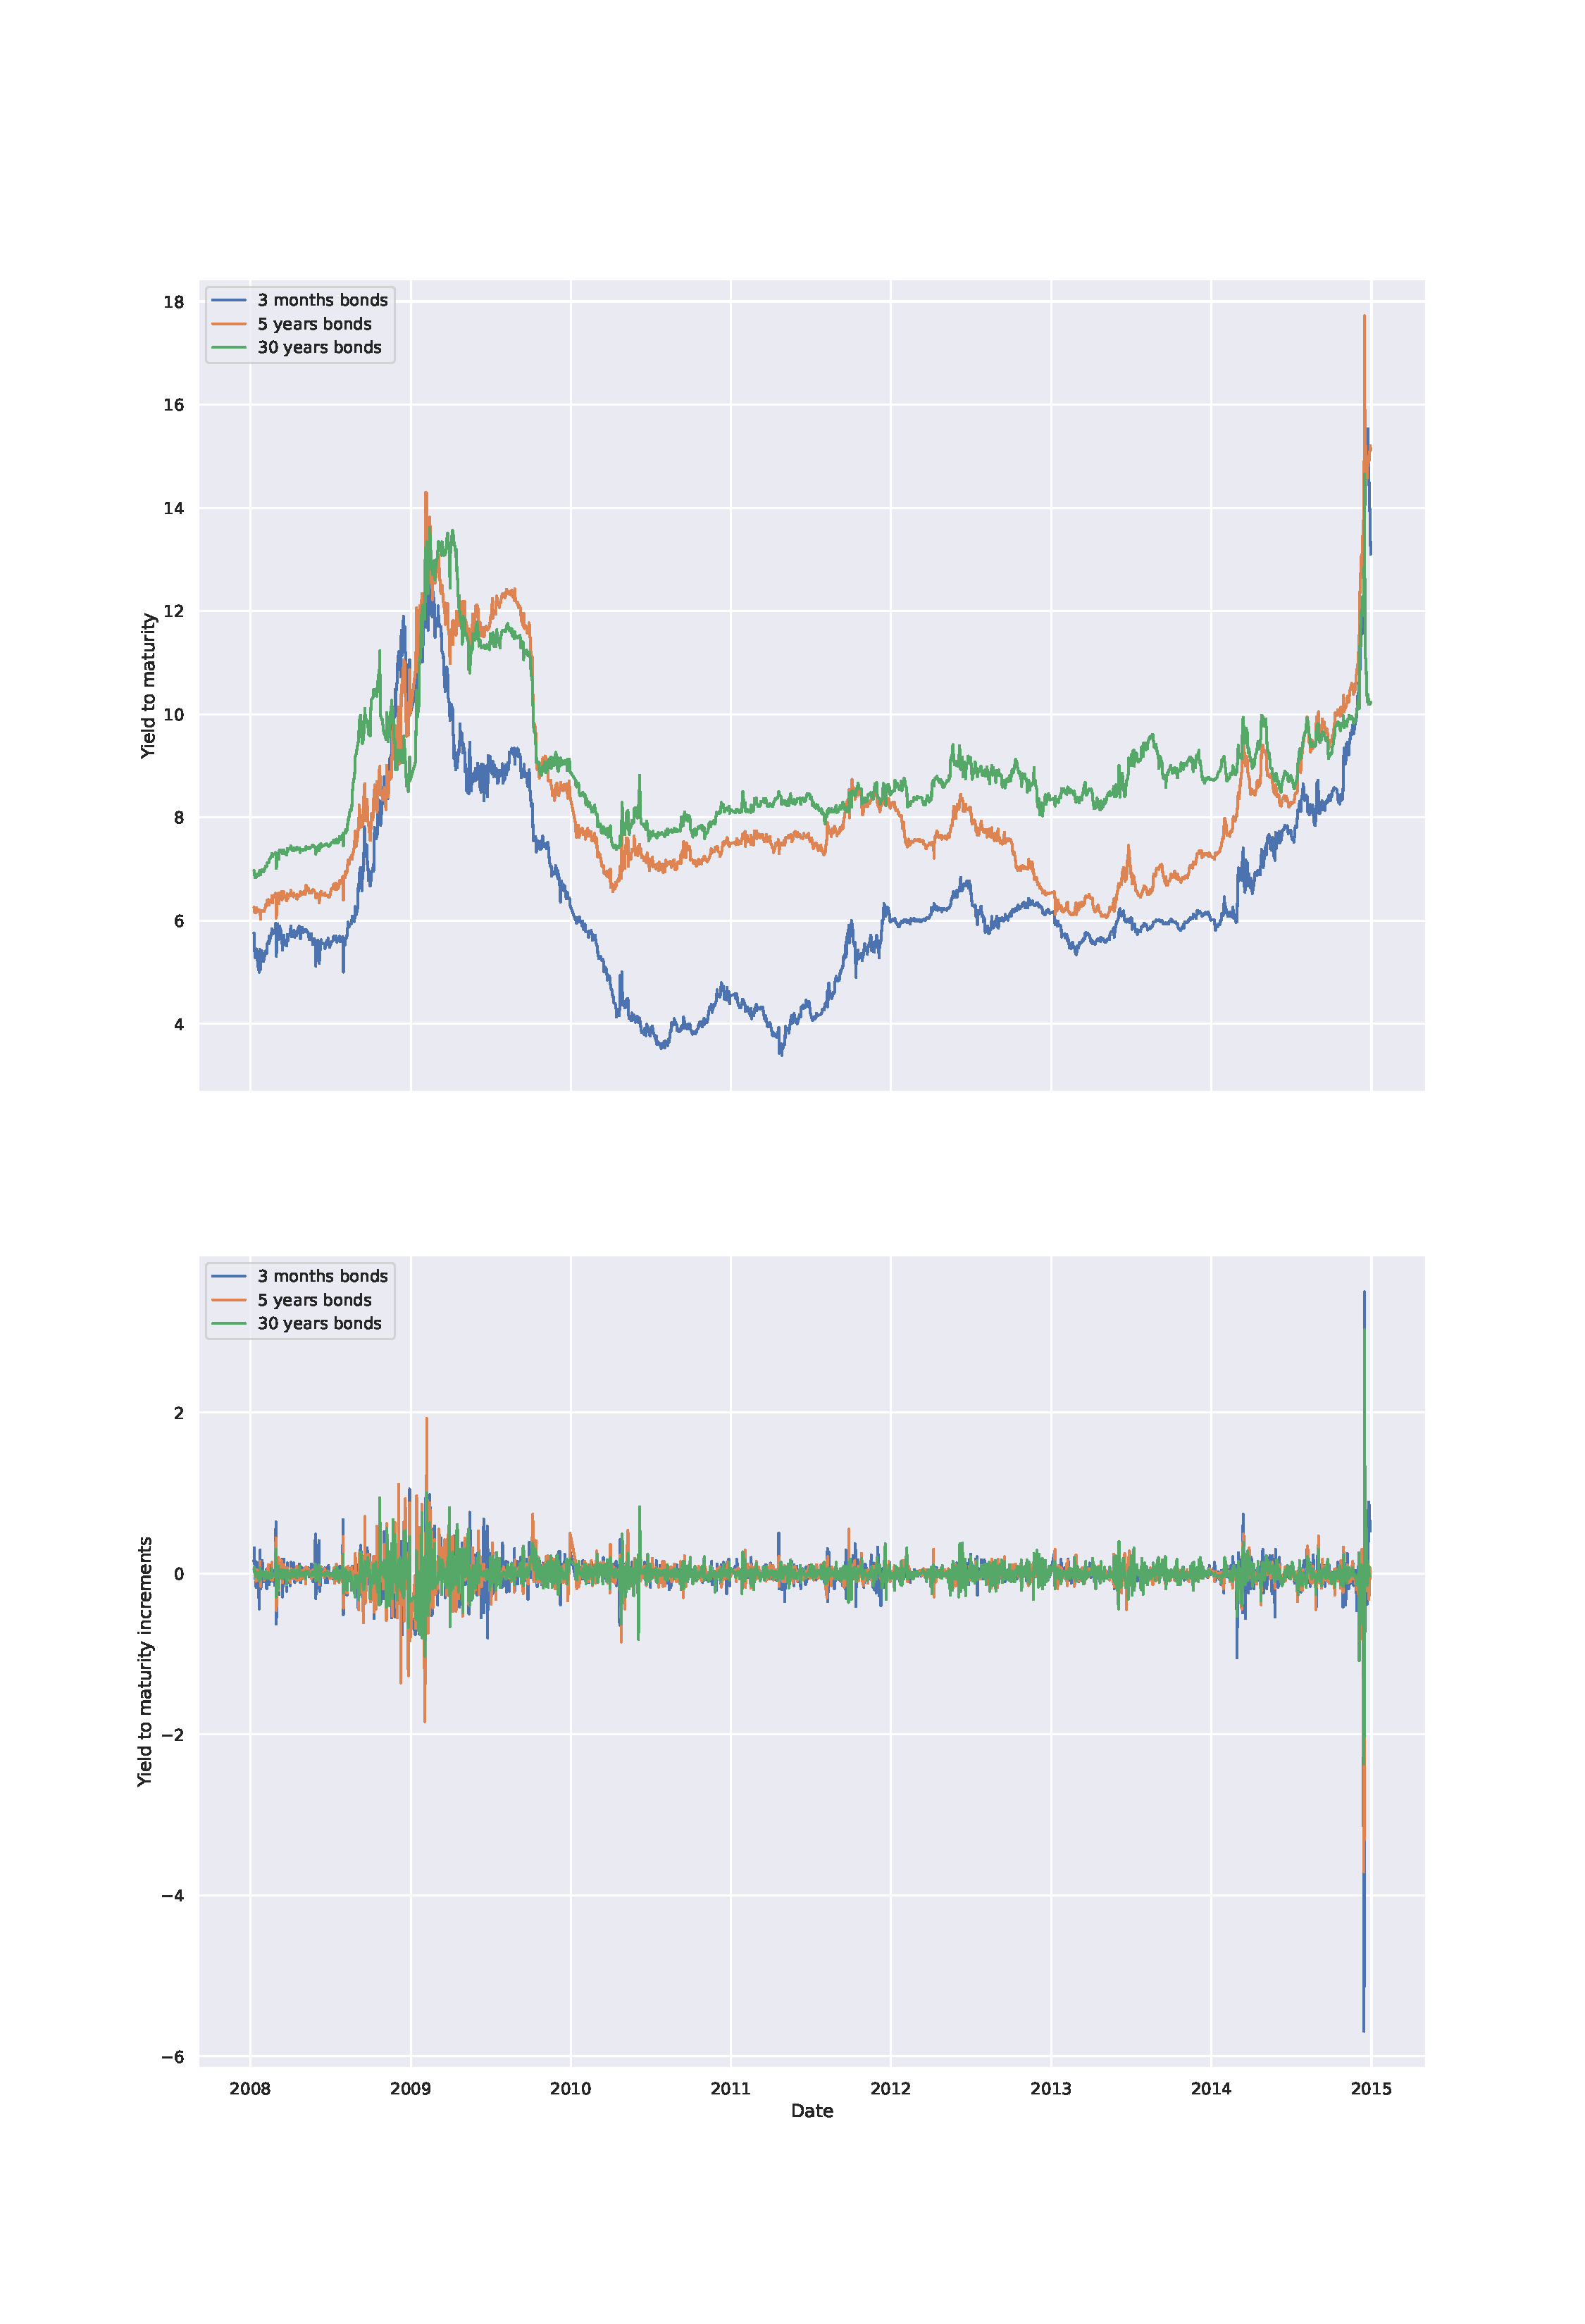
\includegraphics[width=\linewidth]{YTM.pdf}
    \caption{Russian government bond yield to maturity dynamics}
    \label{fig:YTMdynamics}
\end{figure}
    
    \section{Yield Curve Forecasting}
        \section{Yield Curve Forecasting}
    \subsection{Stationarity and cointegration research of the bond yields}
        Stationarity and absence of cointegration are the key assumption for the correctness of many models.
        We shall test the stationarity of the bond yields and the cointegration of the yield curve and the macroeconomic variables.
        \subsubsection{Stationarity}
            In order to test the stationarity of the bond yields, we shall use the \emph{Augmented Dickey-Fuller test} (ADF test).
            The null hypothesis of the test is that the time series is non-stationary.
            The ADF test is a unit root test, which means that it determines how strongly a time series is defined by a trend.
            The test is based on the assumption that the time series is a random walk with drift.
            The test is performed using the \texttt{ur.df} function from the \texttt{urca} package in R.
            The results of the test are presented in Table \ref{tab:adftestForYields} (yields) and Table 
            \ref{tab:adftestForYieldsDifference} (first difference).
            \subimport{results/BondDFtests}{WithoutDiff.tex}
            \subimport{results/BondDFtests}{WithDiff.tex}



        \subsubsection{Cointegration}
            In order to test the cointegration of the yield curve and the macroeconomic variables, we shall use the
            \emph{Johansen test}. The null hypothesis of the test is that the time series are not cointegrated.
            The test is performed using the \texttt{ca.jo} function from the \texttt{urca} package in R.
            The results of the test are presented in Table \ref{tab:johansenTest}.    

            We found out that the bond yields with 3m, 6m, and 9m time to maturity are cointegrated. The obtained results could 
            be explained with the so-called \emph{market segmentation hypothesis}. 
            
            The market segmentation hypothesis states that the yield curve is segmented into different maturity sectors, and the 
            yields in each sector are determined by the supply and demand for bonds in that sector, since the investors could be 
            differentiated by their investment purpose (buying short-term bonds to obtain small but guaranteed revenue, or long-term 
            bonds to hedge against the drop in the interest rate). It implies that the yields with similar maturities can be 
            cointegrated.




    \subsection{Na\"ive approach for the bond yield forecasting}
        \subsubsection{Random walk}
            We assumed the random walk model for the bond yields. The model is defined as follows:
            \begin{equation}\label{eq:RW}
                y_t = y_{t-1} + \epsilon_t.
            \end{equation}
            It is used as a baseline model for the comparison with other models.

        \subsubsection{Auto-ARIMA}
            Later, we assumed the ARIMA model set for the bond yields. The model is defined as follows:
            \begin{equation}\label{eq:ARIMA}
                \Delta^d y_t = \phi_0 + \phi_1 \Delta^d y_{t-1} + \ldots + \phi_p \Delta^d y_{t-p} + \epsilon_t + \theta_1 \epsilon_{t-1} + \ldots + \theta_q \epsilon_{t-q},
            \end{equation}
            where $\epsilon_t$ is the white noise process with zero mean and variance $\sigma^2$, and $\Delta$ is a first difference operator.
            The model is estimated using the \texttt{auto.arima} function from the \texttt{forecast} package in R.

        \subsubsection{Vector Error Correction}
            Later, we assumed the VEC model for the bond yields. The model is defined as follows:
            \begin{equation}\label{eq:VEC}
                \Delta y_{t} = \Pi y_{t-1} + A_0 + A_1 \Delta y_{t-1} + \dots + A_p \Delta y_{t-p} + \epsilon_t. 
            \end{equation}
            where $\epsilon_t$ is the white noise process with zero mean and variance $\sigma^2$.
            The model is estimated using the \texttt{ca.jo} function from the \texttt{urca} package in R.
            
        \subsubsection{Results}
        \
        
            \begin{table}[!htbp]
                \subimport{results}{BondsYresults.tex}
                \label{tab:naiveres}
                \caption{Forecasting results with 1 month horizon and $L^1$ loss (MAE)}
            \end{table}

    \subsection{Nelson-Siegel parametric model}
        \subsubsection{Theoretical description}
            Let us now remind the \emph{Nelson-Siegel model} introduced in \cite{Nelson1987} for the yield curve estimation. The 
            static NS model is defined as follows:
            \begin{equation}\label{eq:NS}
                G(T) = \beta_0 + (\beta_1+\beta_2)\frac{\tau}{T}\left(1-e^{-\frac{T}{\tau}}\right)-\beta_2  e^{-\frac{T}{\tau}},
            \end{equation}
            where $T$ is the time to maturity, $G(T)$ is the yield estimator of the government bonds from the curve basis, 
            and the parameters to be estimated are
            \begin{enumerate}
                \item $\tau$ is the 'typical' time to maturity, 
                \item $\beta_0$ is the long-run of zero-bond yields, 
                \item $\beta_1$ is the mid-run of zero-bond yields, 
                \item $\beta_2$ is the short-run of zero-bond yields.
            \end{enumerate}

            The Nelson-Siegel model offers significant advantages for yield curve estimation and interest rate forecasting. 
            Its simplicity, flexibility, stability, and market insights make it a highly valuable tool.

            The model's simplicity is evident through its use of only a few parameters, making it easy to understand and 
            interpret. Its flexibility allows for capturing both short-term fluctuations and long-term trends in interest 
            rates accurately. The stability of the model is tested and validated across different markets and economic 
            conditions, instilling confidence in its reliability.
            
            Additionally, the Nelson-Siegel model provides valuable insights into market expectations by decomposing the 
            term structure of interest rates. This information is crucial for decision-making and portfolio management. 
            The model's versatility allows for customization and extensions to meet specific needs, further enhancing its 
            applicability.
            
            We shall suggest a modification of the \emph{Dynamic Nelson-Siegel model} introduced in \cite{Diebold2006}.
            First of all, we shall discuss the original DNS model. The functional dependency of the yield curve on the 
            time to maturity $T$ is given by
            \begin{equation}\label{eq:DNS}
                G(t, T) = \beta_0(t) + \beta_1(t)\frac{\tau(t)}{T}\left(1-e^{-\frac{T}{\tau(t)}}\right)-\beta_2(t)  e^{-\frac{T}{\tau(t)}},
            \end{equation}
            where $t$ is the current time, $T$ is the time to maturity at time $t$, $\beta_0(t)$, $\beta_1(t)$, 
            $\beta_2(t)$, and $\tau(t)$ are time-varying parameters. The factors are modeled as AR(1) processes:
            \begin{equation}\label{eq:DNS_AR}
                \begin{aligned}
                    \beta_0(t) &= \beta_0 + \phi_{0,1}(\beta_0(t-1)-\beta_0) + \epsilon_{0,t}, \\
                    \beta_1(t) &= \beta_1 + \phi_{1,1}(\beta_1(t-1)-\beta_1) + \epsilon_{1,t}, \\
                    \beta_2(t) &= \beta_2 + \phi_{2,1}(\beta_2(t-1)-\beta_2) + \epsilon_{2,t}.
                \end{aligned}
            \end{equation}

            \begin{figure}
                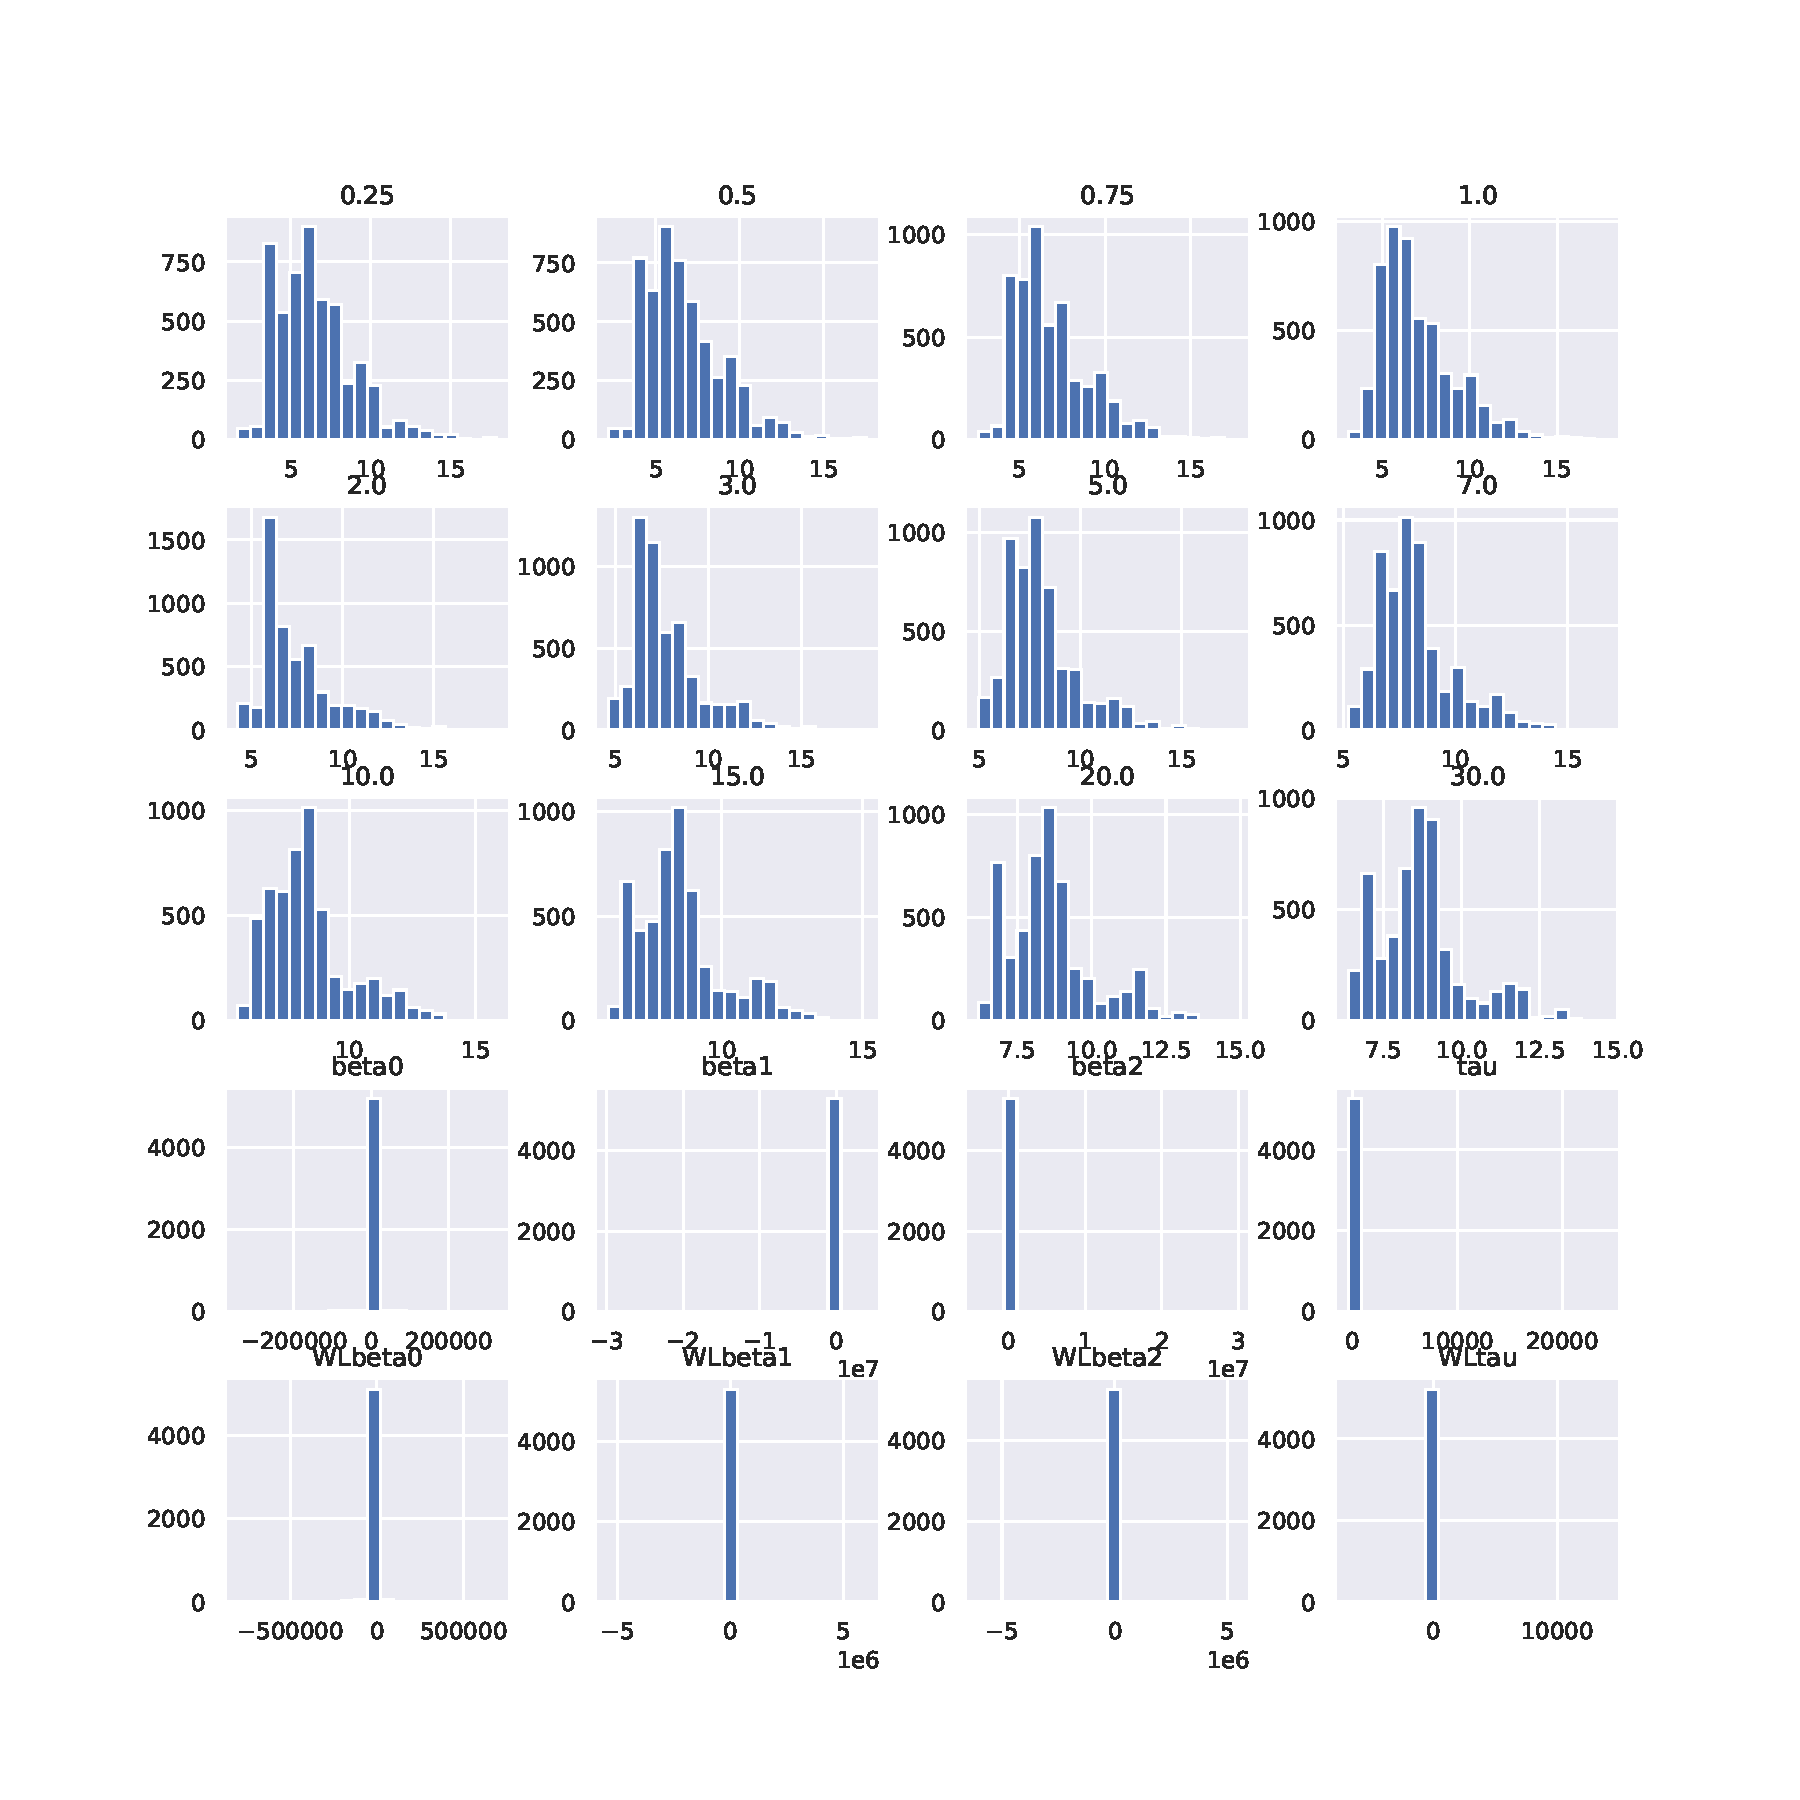
\includegraphics[width=\linewidth]{FactorHist.pdf}
                \caption{Nelson-Siegel factor distribution (with outliers)}
                \label{fig:NSHistOutliers}
            \end{figure}


            \begin{figure}
                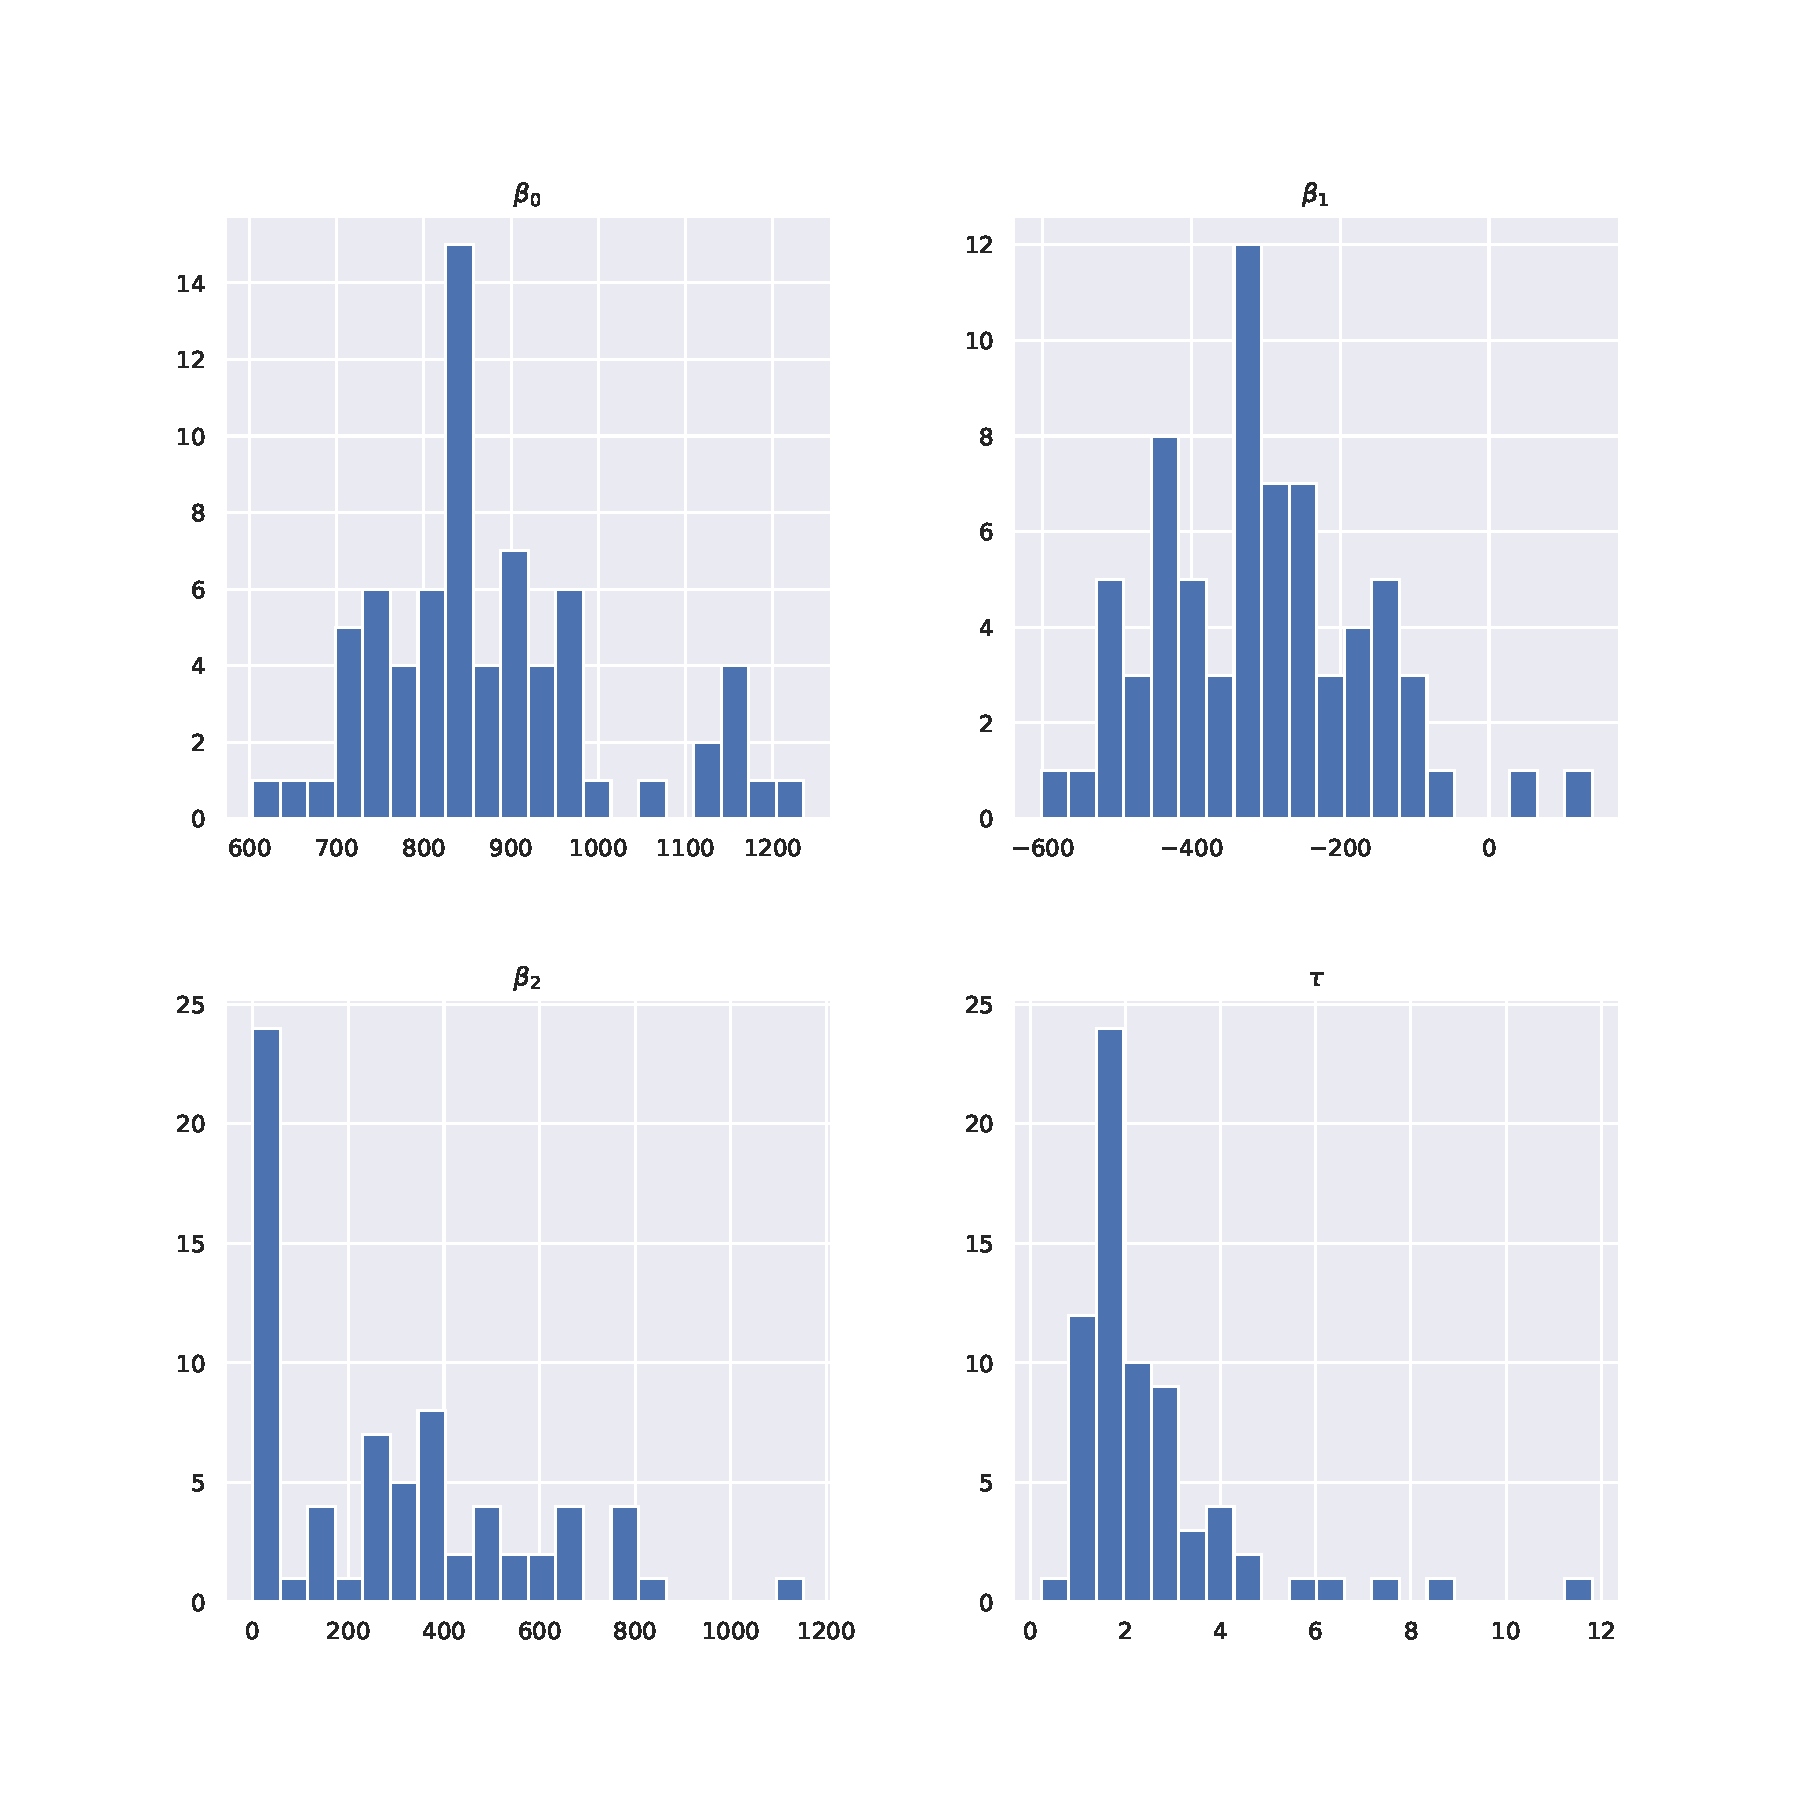
\includegraphics[width=\linewidth]{factorsAfterDrop.pdf}
                \caption{Nelson-Siegel factor distribution (without outliers)}
                \label{fig:NSHistDropped}
            \end{figure}







        \subsubsection{Forecasting results}
            To calibrate the suggested model we followed the steps described below:
            \begin{enumerate}
                \item Using the non-linear least squares method, we estimated the parameters of the static Nelson-Siegel 
                for each day of the sample period.
                \item Given a set of estimated factors, we estimated the parameters of the chosen model using the standard 
                OLS method. The models we used for the factor forecasting:
                    \begin{itemize}
                        \item auto-ARIMA,
                        \item VAR(1),
                        \item Random Walk as a baseline.
                    \end{itemize}
            \end{enumerate}

            After the non-linear least squares optimization, we obtained the factor dynamics found in Figure \ref{fig:factordynamics}.
            \begin{figure}
                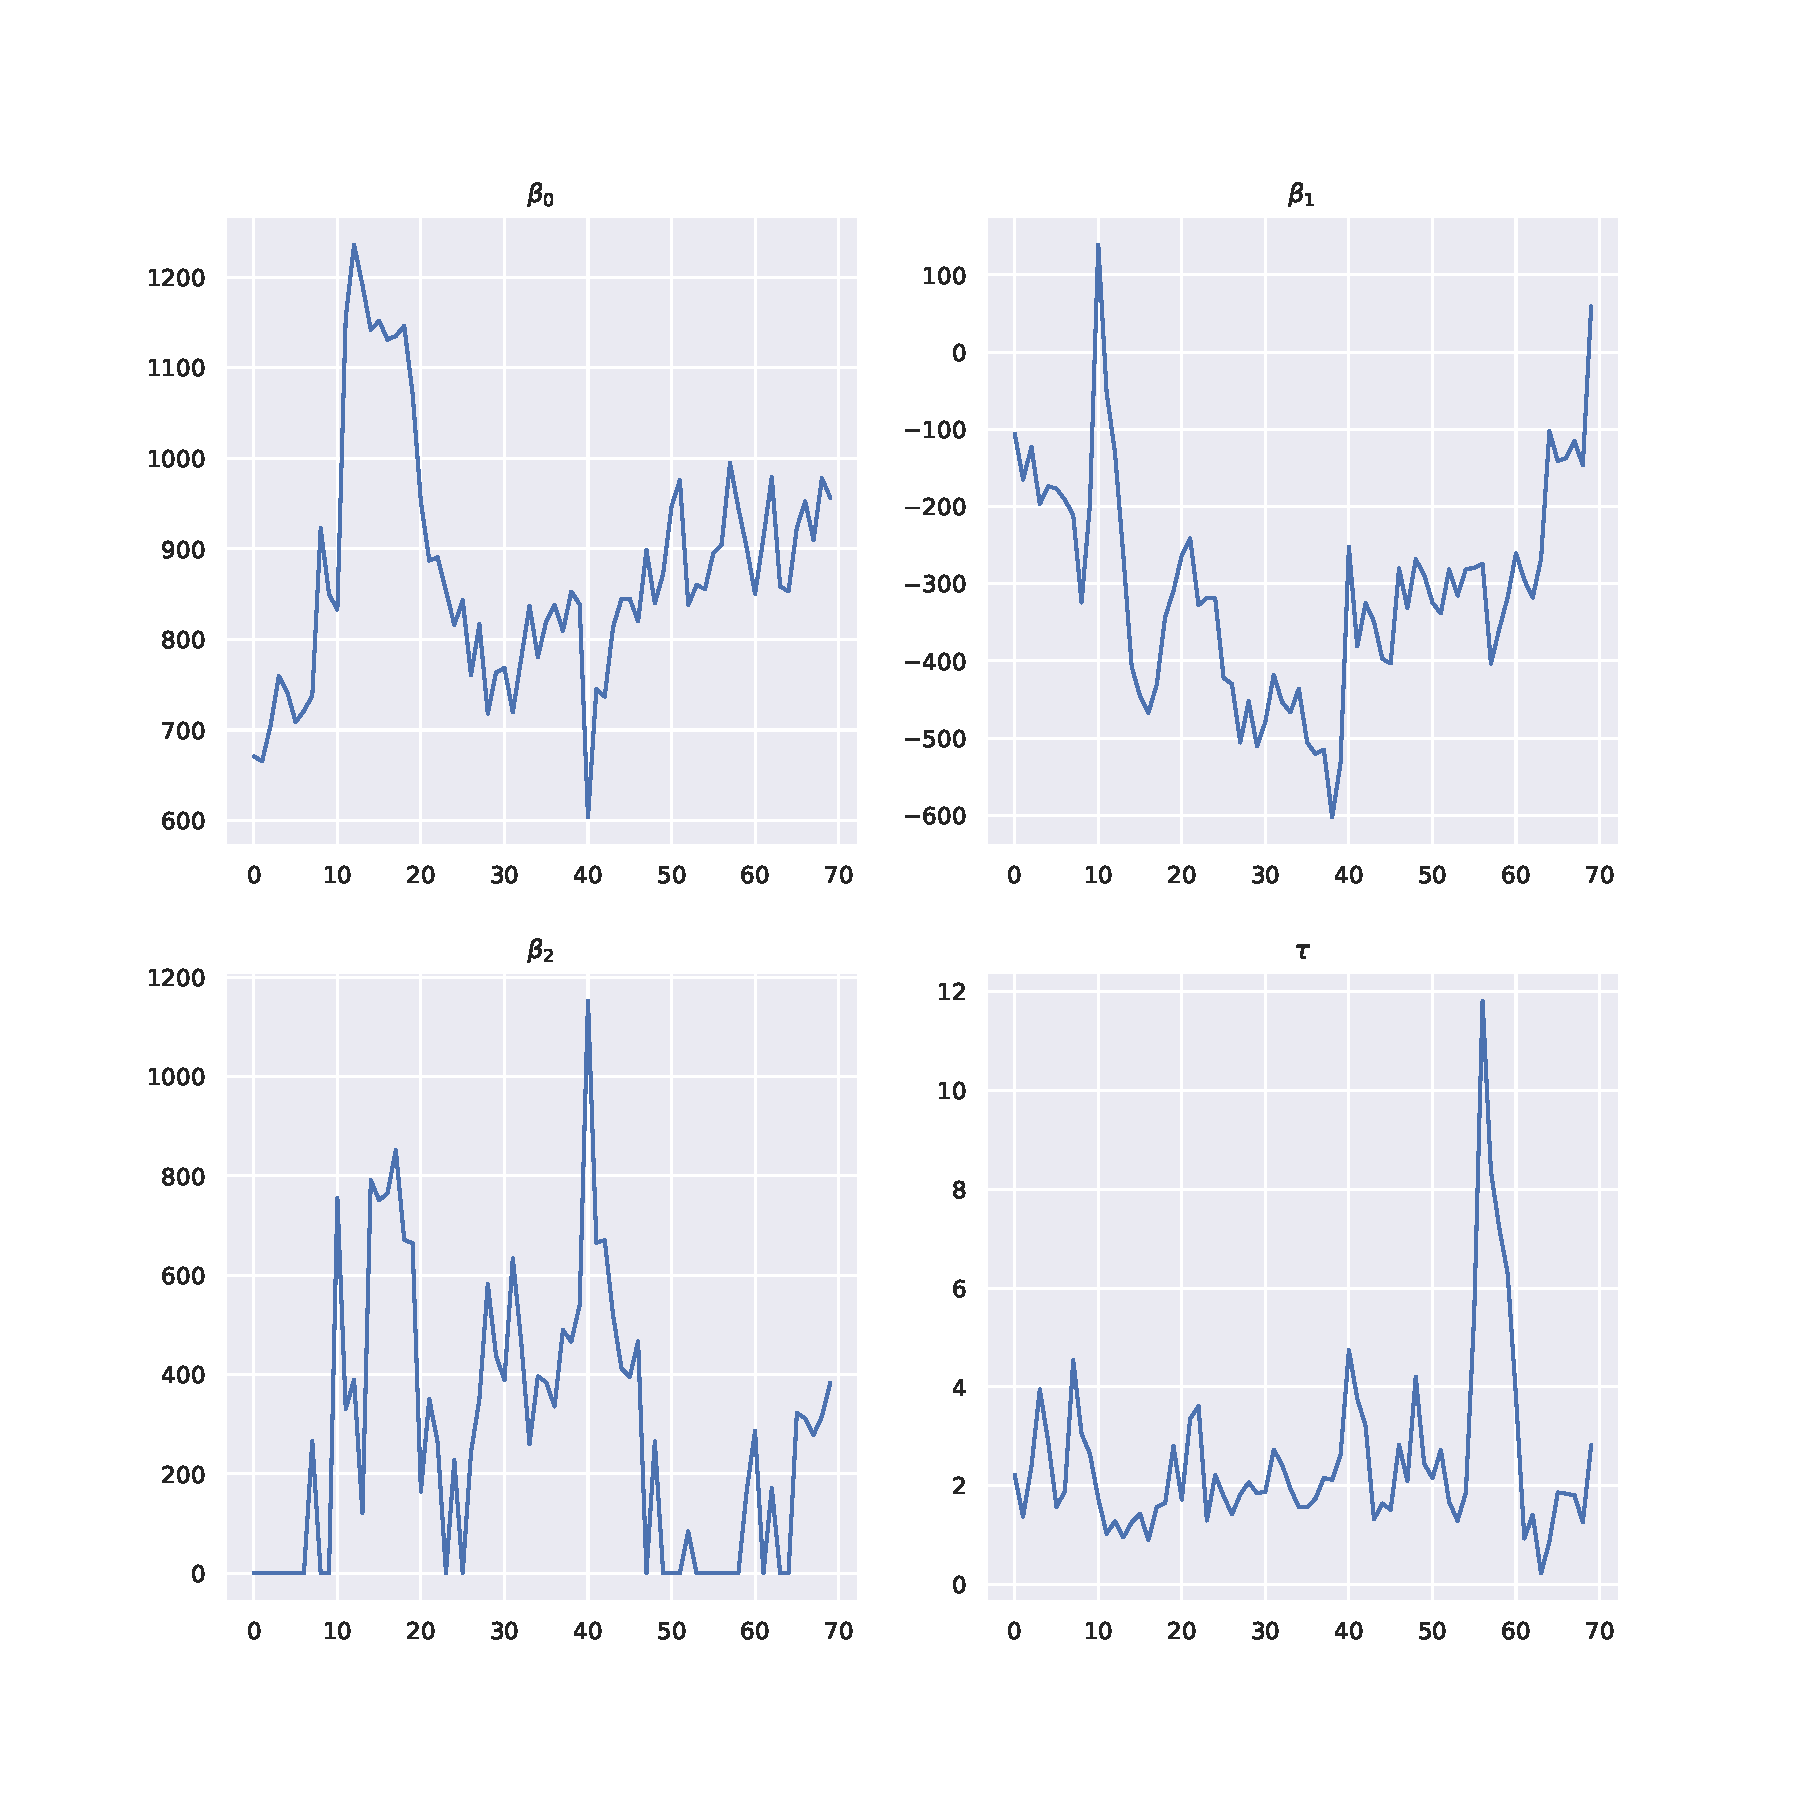
\includegraphics[width=\linewidth]{factors.pdf}
                \caption{Nelson-Siegel factor dynamics}
                \label{fig:factordynamics}
            \end{figure}


            It is possible to use the standard OLS method to estimate the parameters of the DNS model since there is 
            weak stationarity of the factor increments and no cointegration in the calculated time series, see Table \ref{}. 
            \subimport{results/NScoefsStationary}{diffNScoefsStationary}
            \subimport{results/NScoefsStationary}{NScoefsStationary}

            %%%%%%%%%%%%%%
            %%%%%%%%%%%%%%
            %%%%%%%%%%%%%%
            %%%%%%%%%%%%%%
            %%%%%%%%%%%%%%
            %%%%%%%%%%%%%%
            %%%%%%%%%%%%%% Не могу понять где коинтеграция для НС
            %%%%%%%%%%%%%%
            %%%%%%%%%%%%%%
            %%%%%%%%%%%%%%
            %%%%%%%%%%%%%%
            %%%%%%%%%%%%%%
            %%%%%%%%%%%%%%
            %%%%%%%%%%%%%%
            %%%%%%%%%%%%%%
            %%%%%%%%%%%%%%


            It turns out that the best forecast of the NS factors is the constant forecast. The results of the model calibration on a train dataset are presented in Table \ref{tab:DNSresults}.
            \begin{table}[htbp]
                \centering
                
\begin{comment}
     Здесь везде autoARIMA имеет порядок (0,0,0), кроме b2, там (1,0,0). Те в нашей фильтрации коэыыициенты модели - мартингалы.
\end{comment}

\begin{tabular}{|c | c c c|} 
    \hline
    Coefficient & autoARIMA & VAR(1) & RW \\ [0.5ex] 
    \hline
    $\beta_0$ & $53.78356$ & $131.1459$ & $66.3105$ \\ 
    \hline
    $\beta_1$ & $63.31042$ & $143.9235$ & $66.25878$ \\
    \hline
    $\beta_2$ & $133.9688$ & $388.3436$ & $177.1525$ \\
    \hline
    $\tau$ & $1.083687$ & $2.569167$ & $1.328986$ \\
    \hline
\end{tabular}
                \caption{Parameters of the DNS model for 3 different forecasting models.}
                \label{tab:DNSresults}
            \end{table}

    
    \section{Impulse Response Analysis}
        \section{Impulse Response Analysis}\label{sec:IRA}
    We calculated the orthogonal impulse response functions from Nelson-Siegel factors and they turned out to be insignificant (see \cref{fig:nsirf}). This implies that the 
    market segmentation hypothesis holds for the MOEX Russian government bond market.

    \begin{figure}
        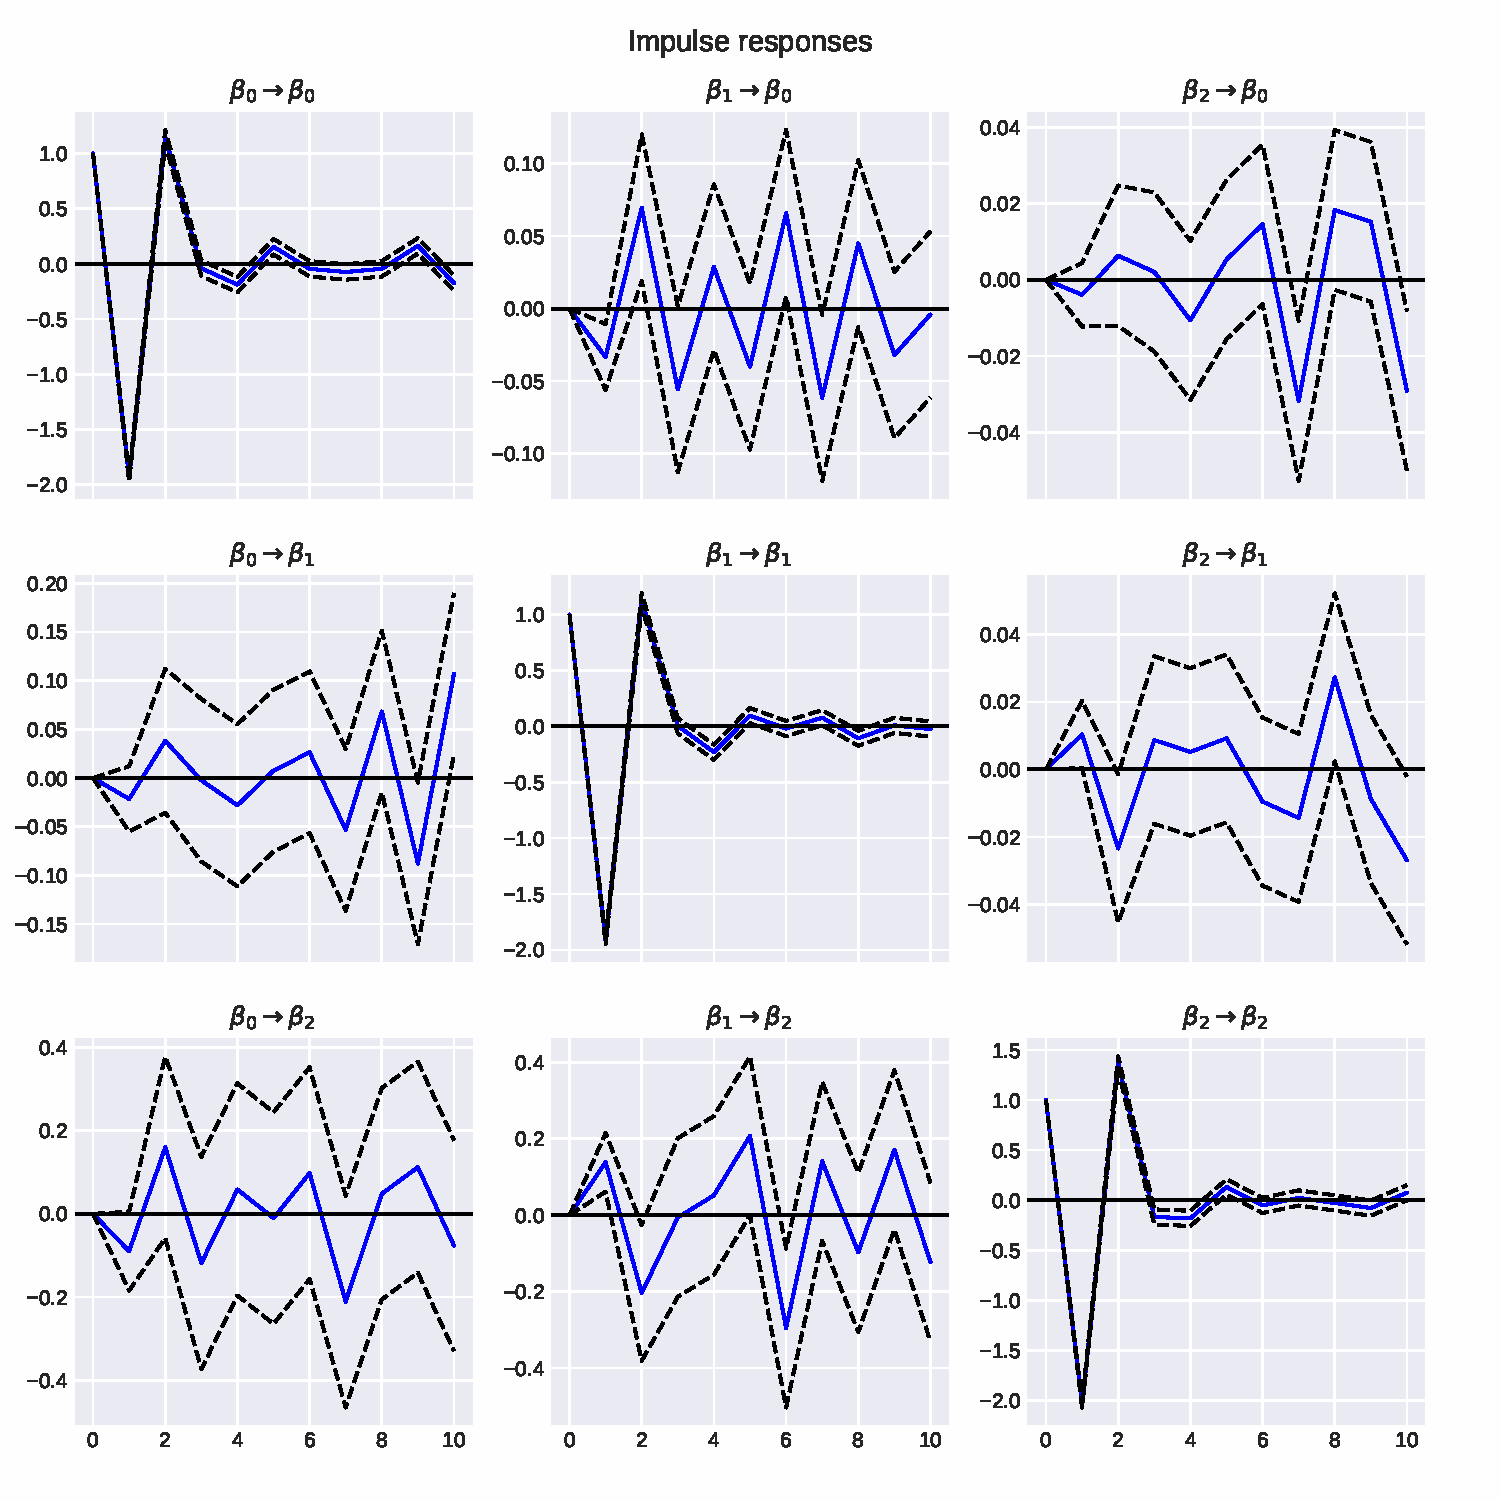
\includegraphics[width=\linewidth]{irfs.pdf}
        \caption{Nelson-Siegel impulse response functions.}
        \label{fig:nsirf}
    \end{figure}


    \section{Structural Breaks Analysis}
        \section{Structural Breaks Analysis}\label{sec:SBA}
    The analysis of the structural breaks in the Nelson-Siegel factor dynamics allows for the identification of periods of volatility or instability 
    in the bond market, which is crucial for investors and policymakers to make informed decisions. This section aims to detect structural breaks in 
    the Nelson-Siegel factor dynamics and examine the timing, magnitude, and nature of these breaks.

    
    Now let us examine the events that happened around the detected structural breaks. We will fix $m=4$ (corresponds to top-4 shocks for 20 years). 
    The detected structural breaks can be found in \cref{tab:detected_breakpoints_obs,tab:detected_breakpoints_dates}. In \cref{tab:optimal_partition_beta0,tab:optimal_partition_beta1,tab:optimal_partition_beta2}, you can find the full list of optimal $(m+1)$-segment partition for $\beta_0$, $\beta_1$, and $\beta_2$ dynamics, respectively.

    \begin{table}[!h]
        \centering
        \begin{tabular}{|c|c|c|c|c|}\hline
            TTM Scale               & First shock & Second shock & Third shock & Fourth shock \\\hline
            Long-run ($\beta_0$)    & 657         & 1384         & 3943        & 4502 \\
            Medium-run ($\beta_1$)  & 938         & 1495         & 2832        & 3524 \\
            Short-run ($\beta_2$)   & 1589        & 2252         & 2869        & 3115 \\\hline
        \end{tabular}
        \caption{Detected structural breaks, numbers of observation detected as breakpoints.}
        \label{tab:detected_breakpoints_obs}
    \end{table}

    \begin{table}[!h]
        \centering
        \begin{tabular}{|c|c|c|c|c|}\hline
            TTM Scale               & First shock & Second shock & Third shock & Fourth shock \\\hline
            Long-run ($\beta_0$)    & 2005-08-30  & 2008-08-08   & 2018-06-21  & 2020-09-09 \\
            Medium-run ($\beta_1$)  & 2006-10-17  & 2009-01-22   & 2014-01-21  & 2016-10-21 \\
            Short-run ($\beta_2$)   & 2009-06-09  & 2012-02-02   & 2014-03-14  & 2015-03-10 \\\hline
        \end{tabular}
        \caption{Detected structural breaks, dates.}
        \label{tab:detected_breakpoints_dates}
    \end{table}


    \begin{landscape}
        \pagestyle{empty}
        \begin{table}
            \centering
            \begin{tabular}{|c|ccccccccccccccccccc|}\hline
                $m$  &      &     &     &     &      &      &      &      &      &      &      &      &      &      &      &      &      &      &      \\\hline
                1  &      &     &     &     &      &      &      &      &      &      &      &      &      &      &      &      &      &      & 4619 \\
                2  &      &     &     &     &      & 1390 &      &      &      &      &      &      &      &      &      &      &      &      & 4619 \\
                3  &      &     & 657 &     &      & 1380 &      &      &      &      &      &      &      &      &      &      &      &      & 4619 \\
                4  &      &     & 657 &     &      & 1384 &      &      &      &      &      &      &      &      &      & 3943 &      & 4502 &      \\
                5  &      &     & 657 &     &      & 1384 &      &      &      &      &      &      &      &      &      & 3943 &      & 4376 & 4622 \\
                6  &      &     & 657 &     &      & 1391 & 1654 &      & 2277 &      &      &      &      &      &      & 3868 &      & 4502 &      \\
                7  &      &     & 657 &     &      & 1391 & 1654 &      & 2277 &      &      &      &      &      &      & 3943 &      & 4376 & 4622 \\
                8  &      &     & 657 &     &      & 1391 & 1654 &      & 2279 &      &      & 2966 &      &      &      & 3945 &      & 4376 & 4622 \\
                9  &      &     & 657 &     &      & 1391 & 1654 &      & 2279 &      &      & 2966 &      & 3525 &      & 3867 &      & 4376 & 4622 \\
                10 &      &     & 657 &     &      & 1391 & 1654 &      & 2279 &      &      & 2966 &      & 3370 & 3616 & 3945 &      & 4376 & 4622 \\
                11 &      &     & 659 &     & 1146 & 1392 & 1654 &      & 2279 &      &      & 2966 &      & 3370 & 3616 & 3945 &      & 4376 & 4622 \\
                12 &      &     & 657 &     &      & 1391 & 1654 &      & 2210 & 2465 & 2714 & 2966 &      & 3370 & 3616 & 3945 &      & 4376 & 4622 \\
                13 &      &     & 659 &     & 1146 & 1392 & 1654 &      & 2210 & 2465 & 2714 & 2966 &      & 3370 & 3616 & 3945 &      & 4376 & 4622 \\
                14 &  322 &     & 657 &     & 1146 & 1392 & 1654 &      & 2210 & 2465 & 2714 & 2966 &      & 3370 & 3616 & 3945 &      & 4376 & 4622 \\
                15 &  322 &     & 654 & 900 & 1146 & 1392 & 1654 &      & 2210 & 2465 & 2714 & 2966 &      & 3370 & 3616 & 3945 &      & 4376 & 4622 \\
                16 &  322 &     & 654 & 900 & 1146 & 1392 & 1654 & 1936 & 2210 & 2465 & 2714 & 2966 &      & 3370 & 3616 & 3945 &      & 4376 & 4622 \\
                17 &  322 &     & 654 & 900 & 1146 & 1392 & 1654 & 1936 & 2210 & 2465 & 2714 & 2966 &      & 3370 & 3616 & 3870 & 4116 & 4376 & 4622 \\
                18 &  322 &     & 654 & 900 & 1146 & 1392 & 1654 & 1936 & 2210 & 2465 & 2711 & 2958 & 3204 & 3450 & 3696 & 3942 & 4188 & 4434 & 4680 \\
                19 &  246 & 492 & 738 & 984 & 1230 & 1476 & 1722 & 1968 & 2214 & 2465 & 2711 & 2958 & 3204 & 3450 & 3696 & 3942 & 4188 & 4434 & 4680 \\
                \hline
            \end{tabular}
            \caption{Optimal $(m+1)$-segment partition for $\beta_0$ dynamics.}
            \label{tab:optimal_partition_beta0}
        \end{table}

        \begin{table}
            \centering
            \begin{tabular}{|c|ccccccccccccccccccc|}\hline
                $m$  &      &     &     &     &      &      &      &      &      &      &      &      &      &      &      &      &      &      &      \\\hline
                1  &      &     &     &     &      &      &      &      &      &      & 2814 &      &      &      &      &      &      &      &     \\
                2  &      &     & 672 &     &      &      &      &      &      &      & 2829 &      &      &      &      &      &      &      &     \\
                3  &      &     & 672 &     &      &      &      &      &      &      &      & 2832 &      & 3524 &      &      &      &      &     \\
                4  &      &     &     & 938 &      & 1495 &      &      &      &      &      & 2832 &      & 3524 &      &      &      &      &     \\
                5  &      &     &     & 938 &      & 1495 &      &      &      &      &      & 2832 &      & 3521 &      &      &      &      & 4619\\
                6  &      &     &     & 938 &      & 1495 &      &      &      &      &      & 2832 &      & 3524 &      &      &      & 4361 & 4607\\
                7  &      &     &     & 917 &      &      & 1772 &      & 2115 &      &      & 2832 &      & 3524 &      &      &      & 4361 & 4607\\
                8  &  246 &     & 672 &     &      &      & 1773 &      & 2115 &      &      & 2832 &      & 3524 &      &      &      & 4361 & 4607\\
                9  &  246 &     & 660 & 959 &      &      & 1772 &      & 2115 &      &      & 2832 &      & 3524 &      &      &      & 4361 & 4607\\
                10 &  246 &     & 660 & 992 &      & 1489 & 1775 &      & 2115 &      &      & 2832 &      & 3524 &      &      &      & 4361 & 4607\\
                11 &  246 &     & 660 & 992 &      & 1489 & 1775 &      & 2115 &      & 2751 & 2997 &      & 3521 &      &      &      & 4361 & 4607\\
                12 &  246 &     & 660 & 992 &      & 1489 & 1775 &      & 2115 &      & 2751 & 2997 &      & 3521 &      &      & 4080 & 4359 & 4605\\
                13 &  246 &     & 660 & 992 &      & 1489 & 1775 &      & 2115 &      & 2751 & 2997 &      & 3521 & 3767 &      & 4080 & 4359 & 4605\\
                14 &  246 &     & 660 & 992 &      & 1489 & 1775 &      & 2115 & 2503 & 2751 & 2997 &      & 3521 & 3767 &      & 4080 & 4359 & 4605\\
                15 &  246 &     & 660 & 992 &      & 1489 & 1775 &      & 2115 & 2503 & 2751 & 2997 & 3256 & 3521 & 3767 &      & 4080 & 4359 & 4605\\
                16 &  246 &     & 660 & 995 & 1243 & 1489 & 1775 &      & 2115 & 2503 & 2751 & 2997 & 3256 & 3521 & 3767 &      & 4080 & 4359 & 4605\\
                17 &  246 & 492 & 738 & 995 & 1243 & 1489 & 1775 &      & 2115 & 2503 & 2751 & 2997 & 3256 & 3521 & 3767 &      & 4080 & 4359 & 4605\\
                18 &  246 & 492 & 738 & 995 & 1243 & 1489 & 1765 & 2011 & 2257 & 2503 & 2751 & 2997 & 3256 & 3521 & 3767 &      & 4080 & 4359 & 4605\\
                19 &  246 & 492 & 738 & 984 & 1230 & 1476 & 1722 & 1968 & 2214 & 2460 & 2706 & 2952 & 3198 & 3444 & 3690 & 3936 & 4182 & 4428 & 4674\\
                \hline
            \end{tabular}
            \caption{Optimal $(m+1)$-segment partition for $\beta_1$ dynamics.}
            \label{tab:optimal_partition_beta1}
        \end{table}

        \begin{table}
            \centering
            \begin{tabular}{|c|ccccccccccccccccccc|}\hline
                $m$  &      &     &     &     &      &      &      &      &      &      &      &      &      &      &      &      &      &      &      \\\hline
                1  &       &     &     &      &      &      &      &      & 2252 &      &      &      &      &      &      &      &      &      &     \\
                2  &       &     &     &      &      & 1589 &      &      & 2223 &      &      &      &      &      &      &      &      &      &     \\
                3  &       &     &     &      &      &      &      &      & 2252 &      &      & 2869 & 3115 &      &      &      &      &      &     \\
                4  &       &     &     &      &      & 1589 &      &      & 2252 &      &      & 2869 & 3115 &      &      &      &      &      &     \\
                5  &   326 &     &     &      &      & 1589 &      &      & 2252 &      &      & 2869 & 3115 &      &      &      &      &      &     \\
                6  &   326 &     &     &      &      & 1589 &      &      & 2252 &      &      & 2869 & 3115 &      &      &      &      &      & 4605\\
                7  &   326 &     &     & 907  &      & 1451 &      &      & 2252 &      &      & 2869 & 3115 &      &      &      &      &      & 4605\\
                8  &   326 &     &     &      &      & 1589 &      &      & 2252 &      &      & 2868 & 3114 & 3374 & 3620 & 3866 &      &      &     \\
                9  &   326 &     &     & 907  &      & 1451 &      &      & 2252 &      &      & 2868 & 3114 & 3374 & 3620 & 3866 &      &      &     \\
                10 &   326 &     &     &      &      & 1589 &      &      & 2252 &      &      & 2868 & 3114 & 3374 & 3620 & 3911 & 4266 &      & 4605\\
                11 &   326 &     &     & 907  &      & 1451 &      &      & 2252 &      &      & 2868 & 3114 & 3374 & 3620 & 3911 & 4266 &      & 4605\\
                12 &   326 &     &     & 907  &      & 1451 &      & 2005 & 2252 &      &      & 2868 & 3114 & 3374 & 3620 & 3911 & 4266 &      & 4605\\
                13 &   326 &     &     & 907  &      & 1451 &      & 1977 & 2223 & 2503 &      & 2868 & 3114 & 3374 & 3620 & 3911 & 4266 &      & 4605\\
                14 &   326 &     &     & 907  &      & 1451 & 1697 & 1977 & 2223 & 2503 &      & 2868 & 3114 & 3374 & 3620 & 3911 & 4266 &      & 4605\\
                15 &   326 &     & 725 & 971  &      & 1451 & 1697 & 1977 & 2223 & 2503 &      & 2868 & 3114 & 3374 & 3620 & 3911 & 4266 &      & 4605\\
                16 &   326 & 572 &     & 908  & 1200 & 1451 & 1697 & 1977 & 2223 & 2503 &      & 2868 & 3114 & 3374 & 3620 & 3911 & 4266 &      & 4605\\
                17 &   326 & 572 &     & 908  & 1200 & 1451 & 1697 & 1977 & 2223 & 2503 &      & 2868 & 3114 & 3374 & 3620 & 3866 & 4112 & 4359 & 4605\\
                18 &   284 & 530 & 776 & 1022 & 1268 & 1514 & 1760 & 2006 & 2252 & 2503 &      & 2868 & 3114 & 3374 & 3620 & 3866 & 4112 & 4359 & 4605\\
                19 &   246 & 492 & 738 & 984  & 1230 & 1476 & 1722 & 1968 & 2214 & 2460 & 2706 & 2952 & 3198 & 3444 & 3690 & 3936 & 4182 & 4428 & 4675\\
                \hline
            \end{tabular}
            \caption{Optimal $(m+1)$-segment partition for $\beta_2$ dynamics.}
            \label{tab:optimal_partition_beta2}
        \end{table}
    \end{landscape}

    Now we shall begin the research of the historical events that happened around the detected structural breaks. 
    Note that the 'date' of the break is estimated approximately, therefore, there could be some discrepancies between 
    the actual date of the suggested event and the estimated date of the detected break.

    \subsection{Long-run yields}
            \paragraph{August 30, 2005} The detected structural break could be associated with three events:
            \begin{enumerate}
                \item The complete stabilization of the Russian economy after the 1998 crisis. In January 2005, free budget 
                balances in the amount of 218.4 billion rubles were transferred to the Stabfond. For the period January-November 
                of this year, the fund was replenished with revenues of the first quarter - in the amount of 210.8 billion rubles, 
                the second quarter - in the amount of 294.4 billion rubles, the third quarter - in the amount of 373.5 billion rubles, 
                October - by 137.7 billion rubles, November - 154.4 billion rubles. The Stabilization Fund began to be formed in Russia 
                on January 1, 2004 in order to reduce the risks associated with unfavorable foreign economic conditions, as well as a 
                tool for sterilizing excess money supply in circulation. It receives huge income of the budget from high oil prices. 
                See \cite{RBK2006}. This event could have led to the decrease in the future supply of the government bonds due to the possible 
                government budget proficit.
                \item The war in Iraq as an indirect cause due to the drastic increase in both spot and futures prices of oil, see 
                \cite{IMF2005}. At the time, the government budget in Russia was calculated using the international oil prices. The 
                increase in oil prices led to the proficit of the government budget, which, in fact, means that the government had more 
                money to spend on the economy (i.e. increase the foreign exchange reserves, reduce government debt and spend more for 
                unforeseen circumstances). Consequently, the emission of the government bonds was reduced, which led to the change in 
                the future supply of the bonds.
                \item United Nations Security Council resolution 1615, adopted unanimously on 29 July 2005, after reaffirming all 
                resolutions on Abkhazia and Georgia, particularly Resolution 1582 (2005), the council extended the mandate of the 
                United Nations Observer Mission in Georgia (UNOMIG) until 31 January 2006.
            \end{enumerate}
            \paragraph{August 08, 2008} The detected structural break could be (and probably is) associated with the start of the 
            Russo-Georgian Conflict and the beginning of the world finanical crisis. Both of these events had 
            a negative impact on the Russian economy. The conflict could have led to the increase in the government spending, which, 
            in turn, led to the increase in the government debt. The world financial crisis led to the decrease in the oil prices, 
            which, in turn, led to the decrease in the government budget proficit. The decrease in the proficit led to the increase 
            in the government debt. Both of these events led to the increase in the future supply of the government bonds. 
            \paragraph{June 21, 2018} The detected structural break could be associated with two events:
            \begin{enumerate}
                \item The Russian Federation experienced a prolonged period of widespread protests from March 2017 to the end of 
                2018, with a focus being on fighting corruption within the government and opposing the increase in the retirement age. 
                The aftermath of these protests could potentially include economic instability due to the disruption of normal business
                operations, increased government spending to address the demands of the protesters, and a loss of investor confidence in 
                the Russian economy. 
                \item 2018 FIFA World Cup. The economic aftermaths of the 2018 FIFA World Cup in Russia included a boost in tourism and 
                hospitality sectors, leading to increased consumer spending and infrastructure development. Additionally, the tournament 
                provided opportunities for small businesses and entrepreneurs, creating a positive impact on the local economy. However, 
                there were also concerns about the long-term utilization of the newly built infrastructure and the potential impact on 
                public finances due to the high costs of hosting the event. 
            \end{enumerate} 
            \paragraph{September 09, 2020} The detected structural break could be associated with first and second waves of COVID-19 
            pandemic. There was a sharp decline in global oil prices, a key source of revenue for Russia, leading to budgetary challenges. 
            Additionally, the pandemic-induced lockdowns and travel restrictions led to a contraction in economic activity, particularly 
            in sectors such as tourism and hospitality. The Russian government implemented several measures, including financial support 
            to businesses and individuals, to reduce the economic impact of the pandemic. The pandemic caused a recession and a range of 
            challenges for businesses and the workforce.

    \subsection{Medium-run yields}
            \paragraph{October 17, 2006} The detected structural break could be associated with two events:
            \begin{enumerate}
                \item The end of the Chechen War and the elimination of a number of militants in Chechnya: Basayev, the main representative 
                of Al-Qaeda in the North Caucasus, the Jordanian Sheikh Abu Omar Al-Seif, Maskhadov's successor, the so-called president 
                of Ichkeria Abdul Halim Saidulayev. The announcement of an amnesty, which, according to the latest data, was used by about 
                five hundred members of illegal armed groups. This could lead to the increase of the nationalistic sentiment, investor confidence, 
                international authority and stability of the economy.
                \item A series of high-profile murders - the first deputy chairman of the Central Bank of Russia, Andrei Kozlov (September 13), 
                the columnist of Novaya Gazeta, Anna Politkovskaya (October 7). This possibly led to the negative aftermaths.
            \end{enumerate}
            \paragraph{January 22, 2009} The detected structural break could be associated with the 2009 Russia-Ukraine gas dispute. In 
            2009, a dispute arose between Russian gas company Gazprom and Ukrainian gas company Naftogaz over accumulating debts for previous 
            gas supplies. The conflict led to a cutoff of Russian gas supplies to Ukraine, which in turn disrupted gas flows to Southeastern 
            Europe and parts of other European countries for 13 days. Despite attempts by the European Union to intervene, the crisis was not 
            resolved until January 18, when Russian Prime Minister Vladimir Putin and Ukrainian Prime Minister Yulia Tymoshenko negotiated a 
            new contract. Following the resolution, gas flows to Europe resumed, but both Russia and Ukraine suffered economic losses, and 
            their reputations as energy supplier and transit country were negatively impacted.
            \paragraph{January 21, 2014} The detected structural break could be associated with two major events: 
            \begin{enumerate}
                \item 2014 Winter Olympics. The economic aftermaths of the 2014 Winter Olympics in Russia included a boost in tourism and 
                hospitality sectors, leading to increased consumer spending and infrastructure development.
                \item The joining of Crimea into the Russian Federation. The event was followed by several economic sanctions imposed by 
                the United States and the European Union, which led to a decline in investor confidence and a reduction in foreign direct 
                investment. Additionally, the Russian economy was negatively impacted by the decline in oil prices and the depreciation 
                of the ruble. Furthermore, the 2014-2016 Russian economic crisis started.
            \end{enumerate}
            \paragraph{October 21, 2016} The detected structural break could be associated with two events:
            \begin{enumerate}
                \item Russian military operation in Syria. It had several impacts on the Russian economy. The defense budget increased significantly 
                to support military operations, diverting funds away from other sectors. However, the operation also led to an increase 
                in nationalistic sentiment, which potentially bolstered the mood of the investors. Overall, the operation 
                had mixed economic effects on the Russian economy.
                \item Allegations of institutionalized doping use by Russian athletes. The Russian doping scandal refers to a series of 
                allegations made against Russia by the World Anti-Doping Agency (WADA) concerning doping violations in multiple sports 
                in the country. The scandal had a negative impact on the reputation of Russian athletes and the country's sports industry, 
                leading to a decline in sponsorship deals and investments.
            \end{enumerate}

    \subsection{Short-run yields}
        We shall not describe the structural breaks for the short-run yields due to the volatile nature of the subject. However, we shall 
        note that the structural breaks for the short-run yields are mostly associated with the events that caused the structural breaks 
        for the medium-run yields.

    \subsection{Forecasting results}
        We decided to divide the dataset into 4 segments which we took from structural analysis of the long-run yields. The results of ARIMA and VAR models restricted to each sector could be found in \cref{tab:structuralARIMA,tab:structuralVAR}, respectively.
        \begin{table}[htbp]
            \centering
            \begin{tabular}{|l|l|l|l|l|l|l|}
            \hline
            Segment            & Factor    & MAPE       & ME       & MAE     & MPE         & RMSE    \\ \hline
            \multirow{4}{*}{0} & $\beta_0$ & 0.0083     & 6.6921   & 6.6921  & 0.0083      & 7.7627  \\ \cline{2-7} 
                               & $\beta_1$ & 0.0155     & 5.8167   & 7.4981  & -0.012      & 7.9825  \\ \cline{2-7} 
                               & $\beta_2$ & 0.1538     & 27.8315  & 30.2092 & 0.1455      & 47.6721 \\ \cline{2-7} 
                               & $\tau$    & 0.1499     & 0.2511   & 0.2511  & 0.1499      & 0.2786  \\ \hline
            \multirow{4}{*}{1} & $\beta_0$ & 0.0076     & -5.9872  & 5.9872  & 0.0076      & 6.2486  \\ \cline{2-7} 
                               & $\beta_1$ & 0.0275     & -5.15    & 6.8624  & 0.0209      & 7.2744  \\ \cline{2-7} 
                               & $\beta_2$ & 21312.0946 & -5.3942  & 55.4278 & -21312.0946 & 55.9851 \\ \cline{2-7} 
                               & $\tau$    & 0.7482     & -1.5317  & 1.5317  & -0.7482     & 1.7142  \\ \hline
            \multirow{4}{*}{2} & $\beta_0$ & 0.0578     & 48.5869  & 48.5869 & 0.0578      & 57.57   \\ \cline{2-7} 
                               & $\beta_1$ & 0.0972     & -15.7947 & 19.6762 & 0.0816      & 27.1274 \\ \cline{2-7} 
                               & $\beta_2$ & 0.1214     & 7.6326   & 27.0065 & -0.0172     & 29.0144 \\ \cline{2-7} 
                               & $\tau$    & 0.0916     & 0.3636   & 0.5129  & 0.069       & 0.5959  \\ \hline
            \multirow{4}{*}{3} & $\beta_0$ & 0.006      & -2.0011  & 5.5102  & -0.0021     & 6.0729  \\ \cline{2-7} 
                               & $\beta_1$ & 0.3471     & 23.9805  & 29.3697 & 0.2982      & 32.2907 \\ \cline{2-7} 
                               & $\beta_2$ & 0.5223     & -93.8611 & 93.8611 & -0.5223     & 95.6724 \\ \cline{2-7} 
                               & $\tau$    & 0.9588     & 1.8988   & 1.8988  & 0.9588      & 1.987   \\ \hline
            \end{tabular}
            \caption{ARIMA forecasting results for the structural NS factors.}
            \label{tab:structuralARIMA}
        \end{table}

        \begin{table}[htbp]
            \centering
            \begin{tabular}{|l|l|l|l|l|l|l|}
            \hline
            Segment            & Factor    & MAPE       & ME       & MAE     & MPE         & RMSE    \\ \hline
            \multirow{4}{*}{0} & $\beta_0$ & 0.0038     & 0.6743   & 3.053   & 0.0009      & 4.3991  \\ \cline{2-7} 
                               & $\beta_1$ &  0.017    &  5.8745   &   8.1959   &  -0.0121    &   8.7872   \\ \cline{2-7} 
                               & $\beta_2$ &   0.1034   &   15.4491  &   20.2472   &   0.0863   &   32.5685   \\ \cline{2-7} 
                               & $\tau$    &  0.1096    &   0.1865  & 0.1865     &  0.1096    &   0.196   \\ \hline

            \multirow{4}{*}{1} & $\beta_0$ &  0.0058    &  -0.3276   &   4.6186   &  -0.0004    &  5.1622    \\ \cline{2-7} 
                               & $\beta_1$ &  0.0355    & -8.4288    &  8.8186    &  0.0339    &  10.2788    \\ \cline{2-7} 
                               & $\beta_2$ &  26187.8876    &  -40.8754   &  47.3524    &  -26187.8563    & 57.5888     \\ \cline{2-7} 
                               & $\tau$    &  0.1294    &  0.0056   &  0.2309    &  0.0279    &  0.2566    \\ \hline

            \multirow{4}{*}{2} & $\beta_0$ &  2.4086    & 2062.9983    & 2062.9983     & 2.4086     &  2109.0292    \\ \cline{2-7} 
                               & $\beta_1$ &  8.8918    & -1986.5645    & 1986.5645     & 8.8918     &  2009.4069    \\ \cline{2-7} 
                               & $\beta_2$ &  30.0551    & -6835.3624    & 6835.3624     & 30.0551     & 7388.3095     \\ \cline{2-7} 
                               & $\tau$    &  4.9541    &  -28.5051   &  28.5051    &  -4.9541    & 30.4631     \\ \hline

            \multirow{4}{*}{3} & $\beta_0$ & 0.0139     & -12.8457    & 12.8457     &  -0.0139    & 14.9255     \\ \cline{2-7} 
                               & $\beta_1$ & 0.134     & -9.6703    &  12.1766    &  -0.1002    &  15.9566    \\ \cline{2-7} 
                               & $\beta_2$ &  0.3394    & -60.4861    & 60.4861     &  -0.3394    &  61.5831    \\ \cline{2-7} 
                               & $\tau$    &  0.3582    &  0.68   &  0.68    & 0.3582     &  0.7972    \\ \hline
            \end{tabular}
            \caption{VAR forecasting results for the structural NS factors.}
            \label{tab:structuralVAR}
        \end{table}

    \section{Conclusion}
\end{document}